\documentclass[a4paper,11pt]{scrartcl}
\usepackage{sansmathfonts}
\usepackage{inconsolata}
\usepackage{hyperref}
\usepackage{listings}
\usepackage{tikz}
\usepackage{tikz-qtree,tikz-qtree-compat}
\usepackage{color}
\usepackage{hhline}
\usepackage[T1]{fontenc} 
\usepackage[utf8]{inputenc}
\usepackage{helvet}
\usepackage{listings}
\usepackage{xcolor}
\usepackage{tabularx}
\usepackage{multicol}
\usepackage{algpseudocode}
\usepackage{amsmath,amssymb,amsthm} 
\renewcommand{\familydefault}{\sfdefault}

\newtheorem{theorem}{Theorem}
\newtheorem{definition}{Definition}

\begin{document}
\section*{Question 1}
\begin{theorem}
    \textsc{Insert} operations do not invalidate a binary search tree.
\end{theorem}
\begin{proof}
Consider the following pseodocode for insertion:

\begin{algorithmic}[1]
\Function{\textsc{Insert}}{node $N$, value $x$}
\If{$N.value < x \land N.RightChild = nil$}
    \State $N.RightChild \gets \textsc{Singleton(x)}$
\ElsIf{$N.value < x \land R.RightChild \neq nil$}
    \State $\textsc{Insert}(N.RightChild, x)$
\ElsIf{$N.value > x \land N.LeftChild = nil$}
    \State $N.LeftChild \gets \textsc{Singleton(x)}$
\ElsIf{$N.value > x \land N.LeftChild \neq nil$}
    \State $\textsc{Insert}(N.LeftChild, x)$
\EndIf
\EndFunction
\end{algorithmic}

Assume that the tree whose root is at $N$ (which may be a subtree of some larger tree) is initially valid. I show that it is thus after any operation, by induction on the recursion in this function.

\begin{itemize}
\item \underline{Base case 1}: If we enter the first case, then the tree whose root is at $N$ initially contains no right subtree. After the operation, it's left subtree is unchanged, and the right subtree consists only of one node whose value is $x$. Since the left subtree is initially valid, and as it's values are less than $N.value$ (as we have assumed $N$ to be initially valid), and since the right subtree is also valid (since it is a singleton), and all the values in the right subtree (i.e. $x$) are greater or equal to $N.value$, thus $N$ remains valid after the operation.
\item \underline{Base case 2}: If we enter the third case, that $N$ is valid after the operation can be shown with an argument symmetrical to the previous one.
\item \underline{Inductive step 1}: If we enter the second case, then, by inductive hypothesis, $N.RightChild$'s subtree will be valid after inserting $x$ into it. Moreover, $N.LeftChild$'s subtree is valid by assumption, and the values in the left subtree are not greater than $N.value$. Finally, by assumption, all values other than $x$ in $N$'s right subtree are greater than $N.value$, and $x$ also satisfies this property in this case. So overall, $N$'s tree is valid after the operation.
\item \underline{Inductive step 2}: If we enter the fourth case, that $N$ is valid after the operation can be shown with an argument symmetrical to the previous one.
\end{itemize}
\end{proof}
\begin{theorem}
    \textsc{Delete} operations do not invalidate a binary search tree.
\end{theorem}
\begin{proof}
Consider the following pseudocode for deletion:

\begin{algorithmic}[1]
\Function{\textsc{Delete}}{node $N$}
\If{$N.RightChild = nil \land N.LeftChild = nil$}
    \State Set $N$'s father's link to $N$ to nil.
\ElsIf{$N.LeftChild = nil \land N.RightChild \neq nil$}
    \State Promote $N.RightChild$ in place of $N$.
\ElsIf{$N.LeftChild \neq nil \land N.RightChild = nil$}
    \State Promote $N.LeftChild$ in place of $N$.
\ElsIf{$N.LeftChild \neq nil \land N.RightChild \neq nil$}
    \State $M \gets \textsc{Successor(N)}$
    \State $\textsc{Swap}(N, M)$
    \State $\textsc{Delete}(N)$.
\EndIf
\EndFunction
\end{algorithmic}

As before I show that, if applied on some node $N$ from a valid tree, then \textsc{Delete} results in a valid tree, by induction on the recursion present in this function. This time, I assume that \textsc{Delete} indeed removes a node from a tree:

\begin{itemize}
\item \underline{Base case 1}: Note that it can easily be shown by induction that, for each node $M \neq N$ in the tree, supposing that $l_M$ is the set of values in the left subtree of $M$ before the operation, $l'_M$ is this set after the operation, and that $r_M$, $r'_M$ are defined symmetrically for the right subtree, then $l_M \subseteq l'_M$ and $r_M \subseteq r'_M$. Now, since the tree is initially valid, we have that $\forall x \in l_M . x < N.value$ and $\forall x \in r_M . N.value < x$. Since $l_M \subseteq l'_M$ and $r_M \subseteq r'_M$, we have that $\forall x \in l'_M . x < N.value$ and $\forall x \in r'_M . N.value < x$. Thus the tree is valid after the operation.
\item \underline{Base case 2}: If we enter the second case, a proof similar to the previous one suffices.
\item \underline{Base case 3}: If we enter the third case, a proof similar to the previous one suffices.
\item \underline{Inductive step}: If we enter the fourth case, then note that:
    \begin{itemize}
    \item Step 9 does not modify the step.
    \item Consider $V = \{v_1, ..., v_N, v_M, ..., v_n\}$, where $v_1 < ... < v_n$, $v_N = N.value$, $v_M = M.value$, the set of values in the tree (note that $v_N$ and $v_M$ are adjacent, as $M = \textsc{Successor(N)}$), and a relation $\prec \in V \times V$. Define $\prec$ to be the smallest total order that includes $v_1 \prec v_2 \prec ... \prec v_M \prec v_N \prec ... \prec v_n$. It is easy to see that, after step 10, the tree is valid w.r.t. $\prec$, although it is not so w.r.t. $<$.
    \item Now, note that step 11 removes $v_M$. Moreover, by the inductive hypothesis, since the tree is initially valid w.r.t. $\prec$, it is also thus after this step. However, note that the tree does not include the value $v_N$, and that, by restricting $\prec$ to $\{v_1, ..., v_n\} \setminus \{v_N\}$, it becomes the same as $<$! This implies that the tree is also valid w.r.t. $<$, as desired.
    \end{itemize}
\end{itemize}

\end{proof}

\section*{Question 2}

The sequence of trees:

\newcommand{\red}[1]{{\color{red}#1\color{black}}}

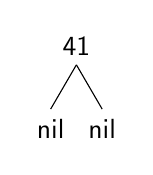
\begin{tikzpicture}
\Tree
    [.41 nil nil ]
\end{tikzpicture}

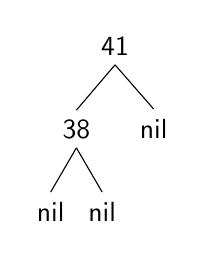
\begin{tikzpicture}
\Tree
    [.41 [.\red{38} nil nil ] nil ]
\end{tikzpicture}

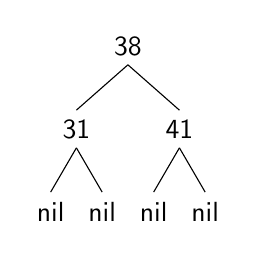
\begin{tikzpicture}
\Tree
    [.38 [.\red{31} nil nil ] [.\red{41} nil nil ] ]
\end{tikzpicture}

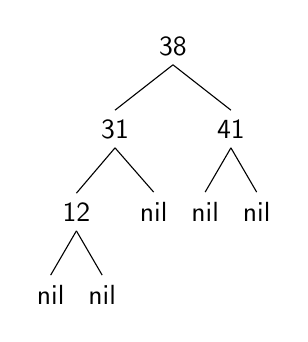
\begin{tikzpicture}
\Tree
    [.38 [.31 [.\red{12} nil nil ] nil ] [.41 nil nil ] ]
\end{tikzpicture}

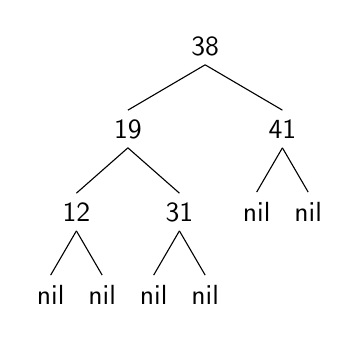
\begin{tikzpicture}
\Tree
    [.38 [.19 [.\red{12} nil nil ] [.\red{31} nil nil ] ] [.41 nil nil ] ]
\end{tikzpicture}

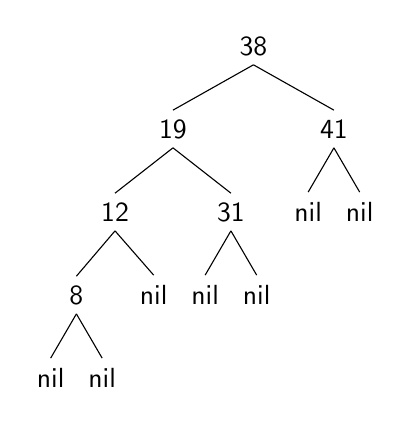
\begin{tikzpicture}
\Tree
    [.38 [.\red{19} [.{12} [.\red{8} nil nil ] nil ] [.{31} nil nil ] ] [.41 nil nil ] ]
\end{tikzpicture}

\section*{Question 3}
\begin{theorem}
    A red-black tree formed by inserting $n \geq 2$ nodes has at least one non-root red node.
\end{theorem}

\begin{proof}
    By induction on $n$:
    \begin{itemize}
    \item \underline{Base case:} For $n = 2$, we note that any red-black tree formed by inserting two values $x \neq y$ has one of two different structures:
        \begin{itemize}
            \item If $x < y$ then: \\
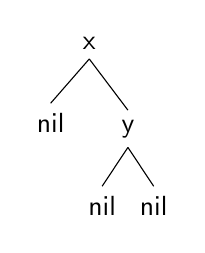
\begin{tikzpicture}
\Tree
    [.x nil [.\red{y} nil nil ] ]
\end{tikzpicture}
            \item If $x > y$ then: \\
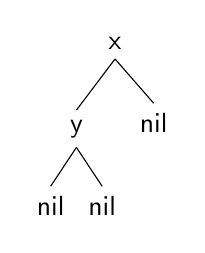
\begin{tikzpicture}
\Tree
    [.x [.\red{y} nil nil ] nil ]
\end{tikzpicture}
        \end{itemize}
            Which obviously satisfy the claim.

    \item \underline{Inductive step:} Note that inserting a node into a red-black tree is done by repeatedly applying various different transformations, according to different case logic. There are 4 different transformations:
        \begin{itemize}
            \item Case 1: \\
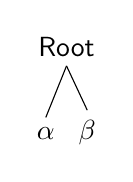
\begin{tikzpicture}
\Tree
    [.\red{Root} {$\alpha$} {$\beta$} ]
\end{tikzpicture}
                Becomes:
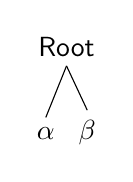
\begin{tikzpicture}
\Tree
    [.Root {$\alpha$} {$\beta$} ]
\end{tikzpicture}
            \item Case 2: \\
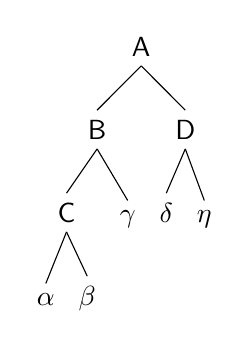
\begin{tikzpicture}
\Tree
    [.A [.\red{B} [.\red{C} {$\alpha$} {$\beta$} ] {$\gamma$} ] [.\red{D} {$\delta$} {$\eta$} ] ]
\end{tikzpicture}
                Becomes:
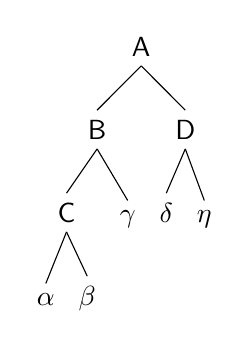
\begin{tikzpicture}
\Tree
    [.\red{A} [.{B} [.\red{C} {$\alpha$} {$\beta$} ] {$\gamma$} ] [.{D} {$\delta$} {$\eta$} ] ]
\end{tikzpicture}
            \item Case 3: \\
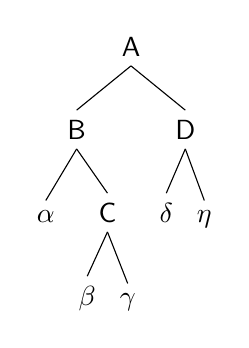
\begin{tikzpicture}
\Tree
    [.A [.\red{B} {$\alpha$} [.\red{C} {$\beta$} {$\gamma$} ] ] [.{D} {$\delta$} {$\eta$} ] ]
\end{tikzpicture}
                Becomes:
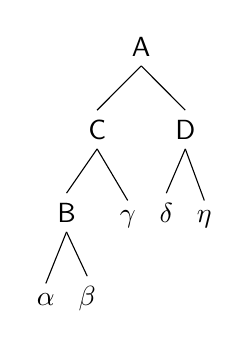
\begin{tikzpicture}
\Tree
    [.A [.\red{C} [.\red{B} {$\alpha$} {$\beta$} ] {$\gamma$} ] [.{D} {$\delta$} {$\eta$} ] ]
\end{tikzpicture}
            \item Case 4: \\
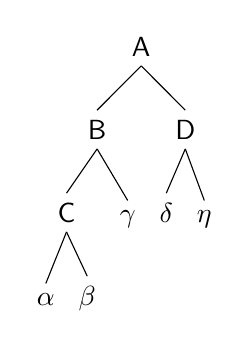
\begin{tikzpicture}
\Tree
    [.A [.\red{B} [.\red{C} {$\alpha$} {$\beta$} ] {$\gamma$} ] [.{D} {$\delta$} {$\eta$} ] ]
\end{tikzpicture}
                Becomes:
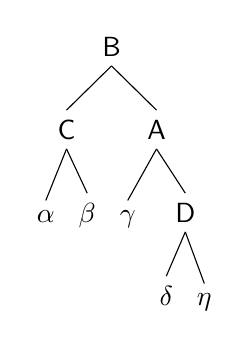
\begin{tikzpicture}
\Tree
    [.B [.\red{C} {$\alpha$} {$\beta$} ] [.\red{A} {$\gamma$} [.D {$\delta$} {$\eta$} ] ] ]
\end{tikzpicture}
        \end{itemize}
        But note that in all cases, if the tree initially has a non-root red node, then it also will have one after the transformation. This means that after any insertion, if the claim holds initially, it also holds at the end.
    \end{itemize}
\end{proof}

\section*{Question 4}
\begin{definition}
    Say that a binary search tree is a "right-chain" if and only if all nodes in the tree lack a left child.
\end{definition}
\begin{theorem}
    Any binary tree with $n$ nodes, whose left subtree has $l$ nodes, and whose left and right subtrees are right-chains, can be turned into a right chain with the same values in $l$ rotations.
\end{theorem}
\begin{proof}
    By induction on $l$, for any $n$:
    \begin{itemize}
        \item \underline{Base case:} For $l = 0$, the tree is already a right chain, so it can be "turned into" a right chain in $0 = l$ operations.
        \item \underline{Inductive step:} For $l > 0$, note that performing a right rotation performed on the root will turn the tree into one whose root's left and right subtrees are right-chains, and whose left subtree has $l-1$ nodes, viz: \\
\tikzset{
    n/.style={draw=none}
}

\begin{tikzpicture}
\Tree
    [.A [.B \edge[n];[.{} ] {$\alpha$} ] {$\beta$} ]
\end{tikzpicture}  \\
            Becomes: \\
\begin{tikzpicture}
\Tree
    [.B {$\alpha$} [.A \edge[n];[.{} ] {$\beta$} ] ]
\end{tikzpicture}  \\
            (where $\alpha$ is a right chain of size $l-1$ and $\beta$ is also a right chain). \\
            Now, by the inductive hypothesis, the resulting tree can be turned into a right-chain with the same elements using $l-1$ rotations. Thus, overall, the initial tree can be turned into a right-chain with the same values using $l$ operations.
    \end{itemize}
\end{proof}
\begin{theorem}
    Any binary tree with $n$ nodes can be turned into a right-chain with the same values in at most $n$ rotations.
\end{theorem}
\begin{proof}
    We prove this by induction on $n$:
    \begin{itemize}
        \item \underline{Base case:} Note that all binary search trees with 1 node are already right-chains (as the sole node has neither left or right child). Thus they can be turned into right-chains with $0 \leq 1 = n$.
        \item \underline{Inductive step:} For $n > 1$, suppose the root's left and right subtrees have $l$ and $r$ nodes respectively. First, apply the inductive hypothesis on the right subtree to turn it into a right-chain in $r-1$ operations. Now, note that by applying a right rotation on the root, we maintain the property that the right subtree is a right-chain, and we reduce the left subtree's size by 1. This implies that by applying at most $l$ further operations, we can turn the tree into a right-chain. Overall this implies that using $l + r - 1 \ leq l + r + 1 = n$ operations we can turn the tree into a right-chain, as required.
    \end{itemize}
\end{proof}
\begin{theorem}
    A right-chain with $n$ nodes can be turned into any binary search tree with the same values in at most $n$ rotations.
\end{theorem}
\begin{proof}
    Use the sequence of rotations that would be used to transform the target binary search tree into a right-chain (which has $n$ rotations at most, by the previous theorem), but reversed, and swapping right-rotations and left-rotations.
\end{proof}

\begin{theorem}
    Any binary tree with $n$ nodes can be turned into any other binary tree with the same values in at most $2n$ rotations.
\end{theorem}
\begin{proof}
    Use the previous two theorems to turn the tree first into a right-chain in $n$ rotations, then into the target tree in another $n$ rotations.
\end{proof}

\section*{Question 5}
After the first splay:

\tikzset{
    n/.style={draw=none}
}
\begin{tikzpicture}
\Tree
    [.2 1 [.10 [.4 \edge[n];[.{} ] [.8 [.6 5 \edge[n];[.{} ] ] \edge[n];[.{} ] ] ] 12 ] ]
\end{tikzpicture} \\
After the second splay: \\

\tikzset{
    n/.style={draw=none}
}
\begin{tikzpicture}
\Tree
    [.5 [.2 1 4 ] [.10 [.8 \edge[n];[.{} ] 6 ] 12 ] ]
\end{tikzpicture} \\

\section*{Question 6}
Take the definiton of right-chains from question 4, and define left-chains analogously. Now, consider a right-chain with $n$ values, viz. $\{ 1, 2, ..., n \}$. Suppose we were to splay the node $n$ with this alternate scheme. By simulating the rotations generated, we can see that, during the splay, the tree is of the following shape: \\
\tikzset{
    n/.style={draw=none}
}
\begin{tikzpicture}
\Tree
    [.1 \edge[n];[.{} ] [.{...} \edge[n];[.{} ] [.n [.{...} k \edge[n];[.{} ] ] \edge[n];[.{} ] ] ] ]
\end{tikzpicture} \\
where $k$ is some value in $\{ 1, 2, ..., n \}$. And the resulting tree after the splay is a left-chain with $n$ values, with the splay costing $\Omega(n)$ operations. Note that then doing a splay on node $1$ now leads again to a cost of $\Omega(n)$, and a right-chain with $n$ values. Alternating these $m$ times gives us a total cost of $\Omega(nm)$.





\end{document}
